% ------------------------------------------------------------------------------
% TYPO3 Version 9.4 - What's New (English Version)
%
% @author	Michael Schams <schams.net>
% @license	Creative Commons BY-NC-SA 3.0
% @link		https://typo3.org/help/documentation/whats-new/
% @language	English
% ------------------------------------------------------------------------------

\section{Changes for Integrators}
\begin{frame}[fragile]
	\frametitle{Changes for Integrators}

	\begin{center}\huge{Chapter 2:}\end{center}
	\begin{center}\huge{\color{typo3darkgrey}\textbf{Changes for Integrators}}\end{center}

\end{frame}

% ------------------------------------------------------------------------------
% #85256 - Install TYPO3 on SQLite

\begin{frame}[fragile]
	\frametitle{Changes for Integrators}
	\framesubtitle{Install TYPO3 on SQLite (1)}

	\begin{itemize}
		\item TYPO3 now supports \href{https://www.sqlite.org}{SQLite},
			a self-contained, lightweight open source SQL database engine
		\item SQLite can be selected during the web-based installation process,
			if PHP module "pdo\_sqlite" is installed and enabled:
	\end{itemize}

	\begin{figure}
		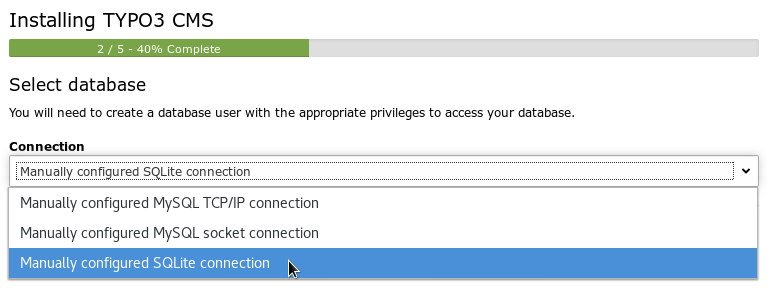
\includegraphics[width=0.65\linewidth]{ChangesForIntegrators/85256-InstallTYPO3OnSQLite.png}
	\end{figure}

\end{frame}

% ------------------------------------------------------------------------------
% #85256 - Install TYPO3 on SQLite

\begin{frame}[fragile]
	\frametitle{Changes for Integrators}
	\framesubtitle{Install TYPO3 on SQLite (2)}

	\begin{itemize}
		\item Database is stored in a single file, which means, TYPO3 instances
			can now run natively in PHP, including the data storage
		\item Using SQLite makes sense for relatively small TYPO3 sites
			or for test and development instances for example
		\item System administrators should take appropriate actions to protect
			the \texttt{*.sqlite} file from unauthorized access, if the file
			is stored inside the web container (depends on type of setup)
	\end{itemize}

\end{frame}

% ------------------------------------------------------------------------------
% #85947 - Page based URL handling

\begin{frame}[fragile]
	\frametitle{Changes for Integrators}
	\framesubtitle{Page-based URL Handling}

	\begin{itemize}
		\item All links generated in the backend and frontend use this field,
			if set
		\item Page-based URL Handling requires a Site Configuration
	\end{itemize}

	\begin{figure}
		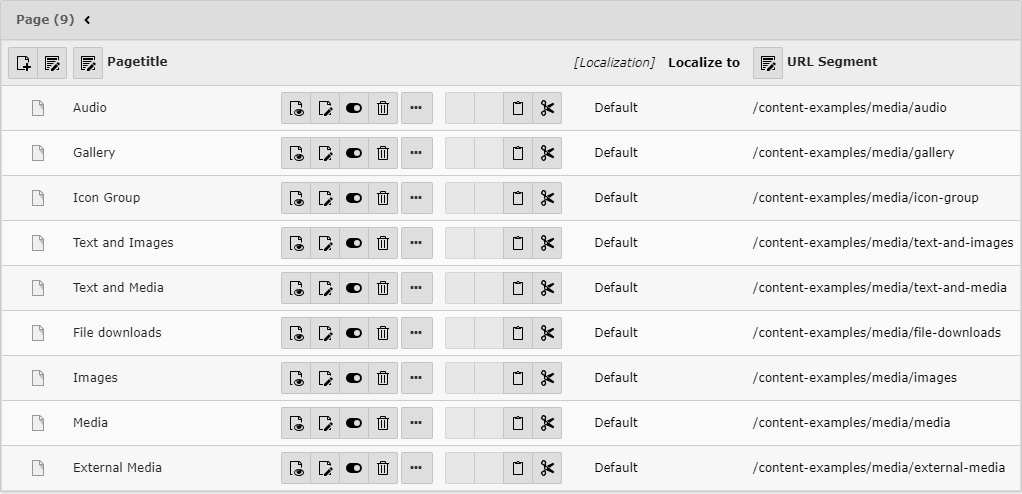
\includegraphics[width=0.7\linewidth]{ChangesForIntegrators/xxxxx-UrlSegments.png}
	\end{figure}

\end{frame}

% ------------------------------------------------------------------------------
% #84729 - New TCA type "slug"

\begin{frame}[fragile]
	\frametitle{Changes for Integrators}
	\framesubtitle{Page-based URL Handling}

	% decrease font size for code listing
	\lstset{basicstyle=\smaller\ttfamily}

	\begin{itemize}
		\item New TCA field type \texttt{slug} has been added
		\item Define parts of a URL path to generate and resolve URLs

		\begin{lstlisting}
'type' => 'slug',
  'config' => [
    'generatorOptions' => [
      'fields' => ['title', 'nav_title'],
      'fieldSeparator' => '/',
      'prefixParentPageSlug' => true
    ]
    'fallbackCharacter' => '-',
    'eval' => 'uniqueInSite'
  ]
		\end{lstlisting}
	\end{itemize}

\end{frame}

% ------------------------------------------------------------------------------
% #44297 - Interval presets for cron command of scheduler task

\begin{frame}[fragile]
	\frametitle{Changes for Integrators}
	\framesubtitle{Scheduler}

	\begin{itemize}
		\item Presets have been added to the Scheduler:

			\begin{itemize}
				\item \texttt{0 9,15 * * 1-5}\tabto{3.8cm}(Mon to Fri at 9:00 and 15:00)
				\item \texttt{0 */2 * * *}\tabto{3.8cm}(every 2 hours)
				\item \texttt{*/20 * * * *}\tabto{3.8cm}(every 20 minutes)
				\item \texttt{0 7 * * 2}\tabto{3.8cm}(every Tuesday at 7:00)
			\end{itemize}

	\end{itemize}

	\begin{figure}
		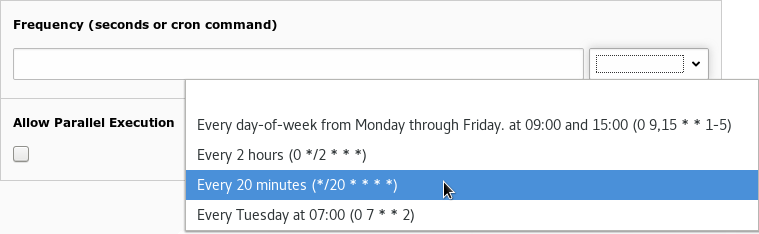
\includegraphics[width=0.80\linewidth]{ChangesForIntegrators/44297-IntervalPresetsInSchedulerTask.png}
	\end{figure}

\end{frame}

% ------------------------------------------------------------------------------
% #83476 - Load merged JS files asynchronous
% #85146 - Read environment variables in TypoScript

\begin{frame}[fragile]
	\frametitle{Changes for Integrators}
	\framesubtitle{TypoScript Changes/Improvements (1)}

	% decrease font size for code listing
	\lstset{basicstyle=\smaller\ttfamily}

	\begin{itemize}
		\item Attribute \texttt{async} is now assigned to the script tag of
			concatenated JS files, if all files have attribute \texttt{async}
			enabled in TypoScript:

			\begin{lstlisting}
config.concatenateJs = 1
page = PAGE
page.includeJSFooter {
  test = path/to/file.js
  test.async = 1
}
			\end{lstlisting}

		\item It is now possible to read environment variables in TypoScript:

			\begin{lstlisting}
# Define default value
myConstant = defaultValue
# Enable overriding by environment variable
myConstant := getEnv(MYCONSTANT)
			\end{lstlisting}

	\end{itemize}

\end{frame}

% ------------------------------------------------------------------------------
% #85550 - Add context check for TypoScript

\begin{frame}[fragile]
	\frametitle{Changes for Integrators}
	\framesubtitle{TypoScript Changes/Improvements (2)}

	% decrease font size for code listing
	\lstset{basicstyle=\smaller\ttfamily}

	\begin{itemize}
		\item The new Context API (see section "Changes for Developers")
			allows integrators to also use this in TypoScript

		\item For example:

			\begin{lstlisting}
10 = TEXT
10.data = context:workspace:id
			\end{lstlisting}

		\item Syntax is: \texttt{context:[aspectName]:[propertyName]}

		\item Arrays are converted to comma-separated lists automatically\newline
			\smaller(ideal for reading details on user groups for example)\normalsize

	\end{itemize}

\end{frame}

% ------------------------------------------------------------------------------
% #86057 - Improved typolink / URL link generation

\begin{frame}[fragile]
	\frametitle{Changes for Integrators}
	\framesubtitle{TypoScript Changes/Improvements (3)}

	% decrease font size for code listing
	\lstset{basicstyle=\smaller\ttfamily}

	\begin{itemize}
		\item With new site-based handling, the de-facto standard \texttt{GET}
			parameter "L" became obsolete
		\item New parameter \texttt{typolink.language} has been introduced

			\begin{lstlisting}
page.10 = TEXT
page.10.value = Link to the page with the ID in the current language
page.10.typolink.parameter = 23
page.20 = TEXT
page.20.value = Link to the page with the ID in the language 3
page.20.typolink.parameter = 23
page.20.typolink.language = 3
			\end{lstlisting}

	\end{itemize}

\end{frame}

% ------------------------------------------------------------------------------
% #85196 - Unify simulate user settings for Backend admins

\begin{frame}[fragile]
	\frametitle{Changes for Integrators}
	\framesubtitle{Simulate User under BE User Settings}

	\begin{itemize}
		\item Administrator users had the option to switch to a different backend
			user ("User Settings → Simulate backend user")
		\item This function has been removed now
	\end{itemize}

	\begin{figure}
		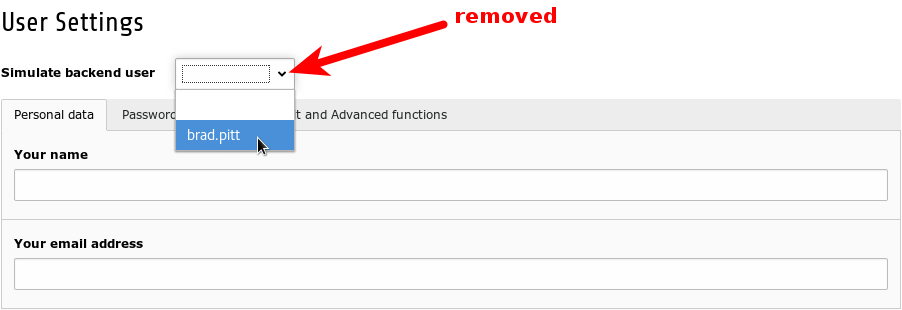
\includegraphics[width=0.80\linewidth]{ChangesForIntegrators/85196-SimulateUserRemovedForAdmins.png}
	\end{figure}

\end{frame}

% ------------------------------------------------------------------------------
% #84133 - Introduce variants

\begin{frame}[fragile]
	\frametitle{Changes for Integrators}
	\framesubtitle{Conditional Variants in \texttt{EXT:form} (1)}

	\begin{itemize}
		\item New feature for extension "Forms": \textit{conditional variants}
		\item Variants can contain conditions and allow changing properties of a
			form element
		\item This way, it becomes possible to manipulate form element values,
			validator and finisher options, etc. based on conditions

	\end{itemize}

\end{frame}

% ------------------------------------------------------------------------------
% #84133 - Introduce variants

\begin{frame}[fragile]
	\frametitle{Changes for Integrators}
	\framesubtitle{Conditional Variants in \texttt{EXT:form} (2)}

	\begin{itemize}
		\item Some typical use cases are for example:

			\begin{itemize}
				\item Translate form element values depending on the current
					frontend language
				\item Set and remove validators depending on the value of
					another form element
				\item Set finisher values depending on the value of a form element.
				\item Hide a form element in certain finishers and on the summary page.
				\item Hide entire pages in the workflow depending on the value of a
					form element.
				\item etc.
			\end{itemize}

		\item \href{https://docs.typo3.org/typo3cms/extensions/form}{Official documentation}
			contains further details and examples

	\end{itemize}

\end{frame}

% ------------------------------------------------------------------------------
% #85355 - Support basic HTML5 fields in FormEngine

\begin{frame}[fragile]
	\frametitle{Changes for Integrators}
	\framesubtitle{HTML5 validation in Backend Fields}

	\begin{itemize}
		\item HTML5 specific field types and attributes are now rendered by
			the FormEngine in the TYPO3 backend
		\item This includes email and numbers, incl. range config, for example
		\item HTML tag attributes are based on the \texttt{eval} TCA configuration
		\item This feature will possibly make custom JavaScript-based processing
			obsolete in the long term
	\end{itemize}

\end{frame}

% ------------------------------------------------------------------------------
% #86001 - Regular Workspace cleanup tasks available via CLI commands

\begin{frame}[fragile]
	\frametitle{Changes for Integrators}
	\framesubtitle{Workspace CLI Commands}

	% decrease font size for code listing
	\lstset{basicstyle=\small\ttfamily}

	\begin{itemize}
		\item TYPO3 now supports two new symfony-based CLI commands to trigger
			regular tasks:

			\begin{itemize}

				\item \texttt{workspace:autopublish}\newline
					Checks for workspaces with auto-publishing configured
					and does a publishing/swapping process.
					\newline

				\item \texttt{cleanup:previewlinks}\newline
					Removes expired previewlinks stored within sys\_preview
					from the database.

			\end{itemize}

		\item Command line execution, for example:

			\begin{lstlisting}
$ typo3/sysext/core/bin/typo3 workspace:autopublish
			\end{lstlisting}

	\end{itemize}

\end{frame}

% ------------------------------------------------------------------------------
% #81430 - Improve TS Template module information on root level list

\begin{frame}[fragile]
	\frametitle{Changes for Integrators}
	\framesubtitle{TypoScript Module Information}

	\begin{itemize}
		\item Overview of TypoScript templates on root page reworked
		\item HTML output uses Fluid templates now
		\item Information shown include page name, template name (with direct
			link to edit the TypoScript record), state (by icon), is root or
			extension template

	\end{itemize}

	\begin{figure}
		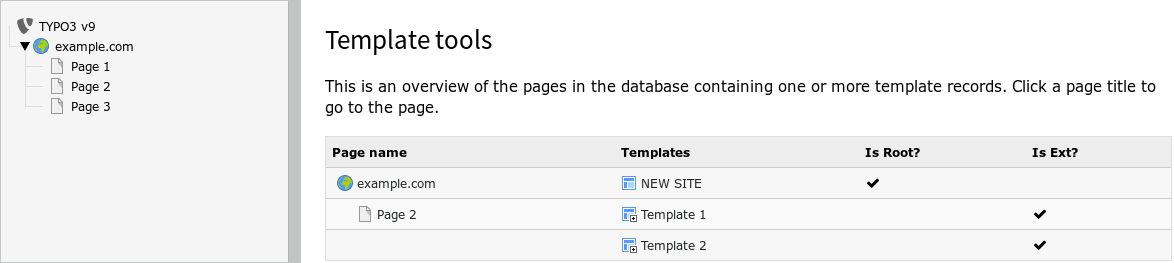
\includegraphics[width=0.80\linewidth]{ChangesForIntegrators/81430-TypoScriptModuleInformation.png}
	\end{figure}

\end{frame}

% ------------------------------------------------------------------------------
% #85393 - Only import extensions from 2015+ into EM

\begin{frame}[fragile]
	\frametitle{Changes for Integrators}
	\framesubtitle{Extension Manager}

	\begin{itemize}
		\item Extensions, older than 10 November 2015 (TYPO3 v7 LTS) are excluded
			from the extension list import
		\item This reduces the database table size by approx. 75\%
	\end{itemize}

\end{frame}

% ------------------------------------------------------------------------------
